% Politecnico di Milano (PoliMi) - School of Industrial and Information Engineering
%
% Copyright 2021 Politecnico di Milano, Italy. NC-BY

\documentclass{Configuration_Files/Template}

%------------------------------------------------------------------------------
%	REQUIRED PACKAGES AND  CONFIGURATIONS
%------------------------------------------------------------------------------

% CONFIGURATIONS
\usepackage{parskip} % For paragraph layout
\usepackage{setspace} % For using single or double spacing
\usepackage{emptypage} % To insert empty pages
\usepackage{multicol} % To write in multiple columns (executive summary)
\setlength\columnsep{15pt} % Column separation in executive summary
\setlength\parindent{0pt} % Indentation
\raggedbottom  

% PACKAGES FOR TITLES
\usepackage{titlesec}
% \titlespacing{\section}{left spacing}{before spacing}{after spacing}
\titlespacing{\section}{0pt}{3.3ex}{2ex}
\titlespacing{\subsection}{0pt}{3.3ex}{1.65ex}
\titlespacing{\subsubsection}{0pt}{3.3ex}{1ex}
\usepackage{color}

% PACKAGES FOR LANGUAGE AND FONT
\usepackage[english]{babel} % The document is in English  
\usepackage[utf8]{inputenc} % UTF8 encoding
\usepackage[T1]{fontenc} % Font encoding
\usepackage[11pt]{moresize} % Big fonts

% PACKAGES FOR IMAGES
\usepackage{graphicx}
\usepackage{transparent} % Enables transparent images
\usepackage{eso-pic} % For the background picture on the title page
\usepackage{subfig} % Numbered and caption subfigures using \subfloat.
\usepackage{tikz} % A package for high-quality hand-made figures.
\usetikzlibrary{}
\graphicspath{{./Images/}} % Directory of the images
\usepackage{caption} % Coloured captions
\usepackage{amsthm,thmtools,xcolor} % Coloured "Theorem"
\usepackage{float}

% STANDARD MATH PACKAGES
\usepackage{amsmath}
\usepackage{amsthm}
\usepackage{amssymb}
\usepackage{amsfonts}
\usepackage{bm}
\usepackage[overload]{empheq} % For braced-style systems of equations.
\usepackage{fix-cm} % To override original LaTeX restrictions on sizes

% PACKAGES FOR TABLES
\usepackage{tabularx}
\usepackage{longtable} % Tables that can span several pages
\usepackage{colortbl}

% PACKAGES FOR ALGORITHMS (PSEUDO-CODE)
\usepackage{algorithm}
\usepackage{algorithmic}

% PACKAGES FOR REFERENCES & BIBLIOGRAPHY
\usepackage[colorlinks=true,linkcolor=black,anchorcolor=black,citecolor=black,filecolor=black,menucolor=black,runcolor=black,urlcolor=black]{hyperref} % Adds clickable links at references
\usepackage{cleveref}
\usepackage[square, numbers, sort&compress]{natbib} % Square brackets, citing references with numbers, citations sorted by appearance in the text and compressed
\bibliographystyle{abbrvnat} % You may use a different style adapted to your field

% OTHER PACKAGES
\usepackage{pdfpages} % To include a pdf file
\usepackage{afterpage}
\usepackage{lipsum} % DUMMY PACKAGE
\usepackage{fancyhdr} % For the headers
\fancyhf{}

% Input of configuration file. Do not change config.tex file unless you really know what you are doing. 
% Define blue color typical of polimi
\definecolor{bluepoli}{cmyk}{0.4,0.1,0,0.4}

% Custom theorem environments
\declaretheoremstyle[
  headfont=\color{bluepoli}\normalfont\bfseries,
  bodyfont=\color{black}\normalfont\itshape,
]{colored}

% Set-up caption colors
\captionsetup[figure]{labelfont={color=bluepoli}} % Set colour of the captions
\captionsetup[table]{labelfont={color=bluepoli}} % Set colour of the captions
\captionsetup[algorithm]{labelfont={color=bluepoli}} % Set colour of the captions

\theoremstyle{colored}
\newtheorem{theorem}{Theorem}[chapter]
\newtheorem{proposition}{Proposition}[chapter]

% Enhances the features of the standard "table" and "tabular" environments.
\newcommand\T{\rule{0pt}{2.6ex}}
\newcommand\B{\rule[-1.2ex]{0pt}{0pt}}

% Pseudo-code algorithm descriptions.
\newcounter{algsubstate}
\renewcommand{\thealgsubstate}{\alph{algsubstate}}
\newenvironment{algsubstates}
  {\setcounter{algsubstate}{0}%
   \renewcommand{\STATE}{%
     \stepcounter{algsubstate}%
     \Statex {\small\thealgsubstate:}\space}}
  {}

% New font size
\newcommand\numfontsize{\@setfontsize\Huge{200}{60}}

% Title format: chapter
\titleformat{\chapter}[hang]{
\fontsize{50}{20}\selectfont\bfseries\filright}{\textcolor{bluepoli} \thechapter\hsp\hspace{2mm}\textcolor{bluepoli}{|   }\hsp}{0pt}{\huge\bfseries \textcolor{bluepoli}
}

% Title format: section
\titleformat{\section}
{\color{bluepoli}\normalfont\Large\bfseries}
{\color{bluepoli}\thesection.}{1em}{}

% Title format: subsection
\titleformat{\subsection}
{\color{bluepoli}\normalfont\large\bfseries}
{\color{bluepoli}\thesubsection.}{1em}{}

% Title format: subsubsection
\titleformat{\subsubsection}
{\color{bluepoli}\normalfont\large\bfseries}
{\color{bluepoli}\thesubsubsection.}{1em}{}

% Shortening for setting no horizontal-spacing
\newcommand{\hsp}{\hspace{0pt}}

\makeatletter
% Renewcommand: cleardoublepage including the background pic
\renewcommand*\cleardoublepage{%
  \clearpage\if@twoside\ifodd\c@page\else
  \null
  \AddToShipoutPicture*{\BackgroundPic}
  \thispagestyle{empty}%
  \newpage
  \if@twocolumn\hbox{}\newpage\fi\fi\fi}
\makeatother

%For correctly numbering algorithms
\numberwithin{algorithm}{chapter}

%----------------------------------------------------------------------------
%	NEW COMMANDS DEFINED
%----------------------------------------------------------------------------

% EXAMPLES OF NEW COMMANDS
\newcommand{\bea}{\begin{eqnarray}} % Shortcut for equation arrays
\newcommand{\eea}{\end{eqnarray}}
\newcommand{\e}[1]{\times 10^{#1}}  % Powers of 10 notation

%----------------------------------------------------------------------------
%	ADD YOUR PACKAGES (be careful of package interaction)
%----------------------------------------------------------------------------

\usepackage{geometry}
\usepackage{tabularx}
\usepackage{booktabs,xltabular}
\usepackage{hyperref}
\usepackage{listings}

%----------------------------------------------------------------------------
%	ADD YOUR DEFINITIONS AND COMMANDS (be careful of existing commands)
%----------------------------------------------------------------------------

% Set uniform margins
\geometry{
  left=0.8in,
  right=0.8in,
  top=1in,
  bottom=1in,
  includehead,
  includefoot
}

%----------------------------------------------------------------------------
%	BEGIN OF YOUR DOCUMENT
%----------------------------------------------------------------------------

\begin{document}

\fancypagestyle{plain}{%
\fancyhf{} % Clear all header and footer fields
\fancyhead[RO,RE]{\thepage} %RO=right odd, RE=right even
\renewcommand{\headrulewidth}{0pt}
\renewcommand{\footrulewidth}{0pt}}

%----------------------------------------------------------------------------
%	TITLE PAGE
%----------------------------------------------------------------------------

\pagestyle{empty} % No page numbers
\frontmatter % Use roman page numbering style (i, ii, iii, iv...) for the preamble pages

\puttitle{
    title= Numerical Analysis for ML \\ Stroke Risk Prediction \\ with Machine Learning Techniques,
    name= {Sara Cavallini, Alberto Eusebio},
    academicyear= {2023-24},
    link= \href{https://github.com/saracavallini01/StrokePrediction}{Click here}

 }

%----------------------------------------------------------------------------
%	PREAMBLE PAGES: ABSTRACT (inglese e italiano), EXECUTIVE SUMMARY
%----------------------------------------------------------------------------
\startpreamble
\setcounter{page}{1} % Set page counter to 1

%----------------------------------------------------------------------------
%	LIST OF CONTENTS/FIGURES/TABLES/SYMBOLS
%----------------------------------------------------------------------------

% TABLE OF CONTENTS
\thispagestyle{empty}
\tableofcontents % Table of contents 
\thispagestyle{empty}
\cleardoublepage

%-------------------------------------------------------------------------
%	MAIN TEXT
%-------------------------------------------------------------------------.

\addtocontents{toc}{\vspace{2em}} % Add a gap in the Contents, for aesthetics
\mainmatter % Begin numeric (1,2,3...) page numbering

% FIRST CHAPTER
% --------------------------------------------------------------------------
\chapter{Scope}

\section{Introduction}

The referenced paper introduces a robust framework for the long term risk prediction of stroke occurences.
A stroke occurs when the blood flow to a specific part of the brain is suddenly interrupted. This interruption leads to the gradual death of brain cells, resulting in disabilities that vary based on the affected brain region. Early identification of stroke symptoms is crucial for effective prediction and fostering a healthy lifestyle, indeed, according to the World Stroke Organization, 13 million people get a stroke each year, and approximately 5.5 million people will die as a result.





\section{Aim}

This research projects is aimed at evaluating the work of Dritsas and Trigka\cite{s22134670}, employing machine learning (ML) techniques to develop and evaluate multiple models, aiming to create a robust framework for long-term stroke risk prediction. The above mentioned study's main contribution is the development of a stacking method that demonstrates high performance, validated by various metrics including AUC, precision, recall, F-measure, and accuracy. 

% SECOND CHAPTER
% --------------------------------------------------------------------------
\chapter{Stroke Risk Prediction Framework Main Aspects}

\section{Project Scope and Methodological Framework}

In this section, we present the project scope, our methodology, and how our work differs from the original paper by Dritsas and Trigka. Our primary goal was to replicate and evaluate their study on stroke prediction using machine learning techniques. We began by preprocessing the data, following similar steps as outlined in the paper, including handling missing values, filtering out patients and augmenting the dataset.

We conducted an extensive Exploratory Data Analysis (EDA) to ensure the integrity and quality of the data. Our EDA confirmed that the data distribution and percentages matched those reported in the original study, indicating accurate preprocessing.

\section{Dataset Augmenting}

We addressed the class imbalance in the dataset using the SMOTE oversampling technique, unlike the original study, which only augmented the training dataset. This adjustment was made to ensure a balanced representation of classes in the entire dataset.

\section{Feature Ranking}

In terms of feature ranking, we applied the random forest classifier and information gain ranking, which corroborated the original study's findings on the importance of age, BMI, and glucose level in stroke prediction.

\section{Model Training}

Finally, we trained multiple models, tuning hyperparameters using GridSearchCV to identify the best-performing models. We implemented and evaluated both stacking and voting methods as described in the original study, comparing the results against the reported metrics. Our evaluation revealed some inconsistencies in the reported performance metrics, which we discuss in the following sections.

\section{Best Practices}

To address some of the discrepancies between the paper methods and the recommended best practices, we have developed two version of the notebook that we will refer to as version A and B. The first tries to replicate the paper steps, while the latter introduces variations and best practices to address some of the problems that we have found while analyzing the paper.


% THIRD CHAPTER
% --------------------------------------------------------------------------
\chapter{Methodology}

\section{Exploratory Data Analysis}

\subsection{Data Pre-processing}

\subsubsection{Selected Dataset}

As mentioned in the paper, the dataset was obtained from \textbf{\href{https://www.kaggle.com/datasets/fedesoriano/stroke-prediction-dataset}{Kaggle}} due to its extensive collection of partcipants, totaling 3254. The dataset can be accessed at the following link: \url{https://www.kaggle.com/datasets/fedesoriano/stroke-prediction-dataset}.
To prepare the data for model training, we've followed a systematic approach to clean and preprocess the dataset. This has involved several key steps to ensure data quality and consistency.

\subsubsection{Data Cleaning}

The first step was to drop unnecessary columns, in our case the only column we had to remove because it was not useful for our purpose was the one containing the 'ids' of the participants.
Subsequently, we identified and handled missing or null values in the dataset. Specifically, the BMI column contained 201 N/A values, which we decided to remove in version A to maintain data integrity but, in many cases, since the number of null values is high compared to the total number of samples, data imputation is also an option and this is what we have done in the notebook containing version B. In line with the original paper, since it clearly states that only participants above 18 years old were considered, we have kept only patients above 18 years old in both versions, removing younger ones to ensure consistency in the age demographics. Additionally, in version A we filtered out patients with unknown smoking status and the ones having 'Other' in the gender feature, to reduce uncertainty in the data.
We also tried to eliminate any duplicates but saw that the dataset lacks them.

However, as it appears from our analysis, the amount of null values are all concentrated in the BMI class and they account for up to 16.06\% of the stroke values, so dropping them will consist in a significant information loss. In version B of the notebook, we have decided to impute these values with the mean of the category BMI.
Similarly, the single 'Other' label in the gender category was set to the most frequent label in the class: 'female'. Handling the imputation of the 'Unknown' label in the smoking status feature is equally important, as these samples account for 13.46\% of the stroke class samples and this is a significant percentage and we should be careful in removing it.
Since the 'Unknown' label is the second largest one for the class in the dataset, simply imputing it to the majority class would not capture all the variance of the dataset, so we have decided to train a Random Forest Classifier to reclassify this label. It is important to note that we did not use the stroke column when training the classifier, not to introduce bias in the dataset itself.

\subsubsection{Outliers}

In the original study, the authors removed the single lowest BMI value, which we also replicated to maintain consistency. We conducted further analysis to identify and address any other significant outliers that could skew the model results, ensuring a robust dataset for training. In version A we have removed the single lowest value of the BMI, while in version B we have adopted the Inter Quartile Method to classify and remove outliers both in the BMI and average glucose level categories.

\subsubsection{Categorical Encoding}

Categorical features in the dataset were encoded using one-hot encoding for multi-class features. This approach was chosen to facilitate the effective use of categorical data in machine learning models. One-hot encoding was used to prevent any ordinal relationship assumptions. Furthermore, the numerical features such as BMI, age and average glucose level were normalized.

\subsubsection{Addressing Imbalances}

The original paper highlighted a class imbalance between smokers and non-smokers, which we confirmed during our analysis. To address this, we used the SMOTE (Synthetic Minority Over-sampling Technique) method to balance the dataset by oversampling the minority class, the 'no\_stroke' class. In the original study, the resampling was performed on the entire dataset, so we have replicated this procedure in notebook A. However, since is common practice to resample only the training dataset, in notebook B we have done so. This choice was motivated by the need for a clean test dataset, to evaluate the performances of the algorithms on.

We also compared SMOTE with SMOTENC (SMOTE for Nominal and Continuous features), a variation that considers categorical features while generating synthetic samples. In fact, applying SMOTE on the dataset corrupts the one-hot encoded features that must be then rounded down to avoid multi-class definition errors that arise when resampling the dataset. In fact, consider the tuple (0, 0.32, 1) obtained through resampling and belonging to the smoking-status category, it makes no sense to say that the patient belongs to the 'smoking' category and also partially to the 'never smoked' one.

\subsubsection{Data Splitting}

The dataset was randomly split into two parts, for training and test. The training subset includes 80\% of the data in the dataset, while the testing dataset accounts for 20\%. As stated before, while in notebook A we have performed resampling on the whole dataset, in notebook B we have decided to oversample only the training set. This led to significantly different performance results in the two dataset.

\subsection{Graphs}

In this section, we analyze the correlation between different features and present various graphs to illustrate these relationships. Each graph is accompanied by an explanation of the results obtained and their implications for stroke prediction.

\subsubsection{Imbalanced Dataset}

In this first part, we are going to present some of the graphs belonging to the imbalanced dataset.
\ref{fig:dataset_imbalance} shows clearly the underrepresentation of the stroke class.

\begin{figure}[h]
\centering
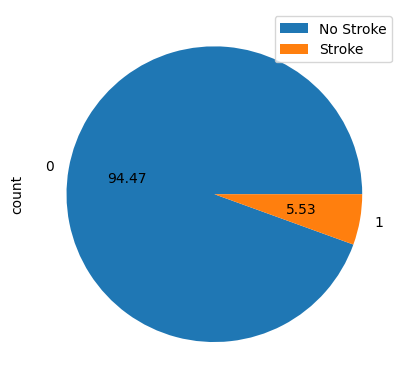
\includegraphics[scale=0.4]{Images/imbalance_pie.png}
\caption{Imbalance distribution}
\label{fig:dataset_imbalance}
\end{figure}

\begin{figure}[ht]
\centering
\begin{subfigure}[b]{\linewidth}
\centering
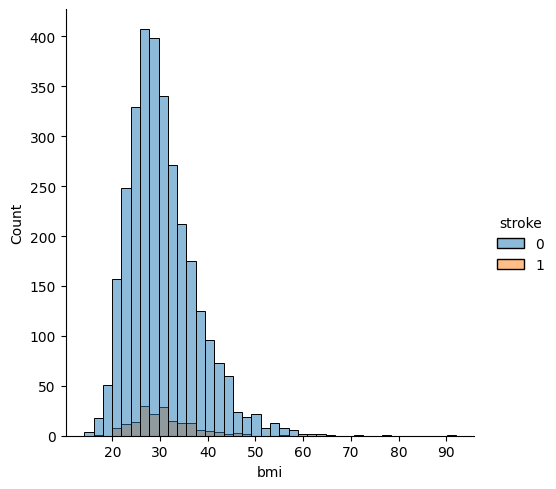
\includegraphics[scale=0.4]{Images/bmi_distribution.png}
\caption{BMI distribution}
\label{fig:bmi_distribution}
\end{subfigure}

\begin{subfigure}[b]{\linewidth}
\centering
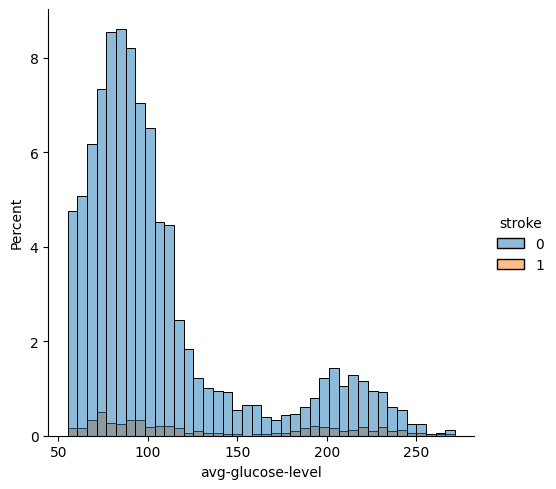
\includegraphics[scale=0.4]{Images/glucose_distribution.png}
\caption{Average Glucose level distribution}
\label{fig:glucose}
\end{subfigure}

\begin{subfigure}[b]{\linewidth}
\centering
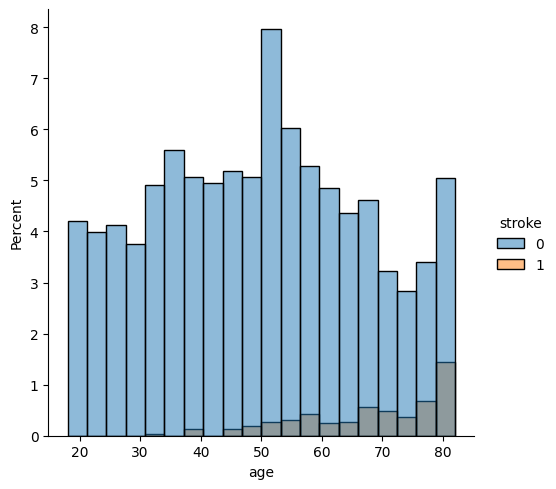
\includegraphics[scale=0.4]{Images/age_distribution.png}
\caption{Age distribution}
\label{fig:age_distribution}
\end{subfigure}
\end{figure}

We start by plotting the distribution of the numerical features inside the dataset. \ref{fig:bmi_distribution}, \ref{fig:glucose}, \ref{fig:age_distribution} are the plots of the distributions for the BMI, the average glucose level and age categories. Interestingly, the average glucose level category has two peaks.

\begin{figure}[ht]
\begin{subfigure}[b]{\linewidth}
\centering
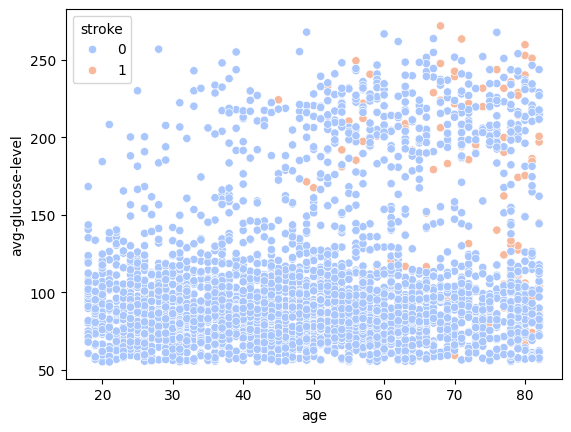
\includegraphics[scale=0.4]{Images/age_glucose_plot.png}
\caption{Age-Glucose correlation plot}
\label{fig:age_glucose}
\end{subfigure}

\begin{subfigure}[b]{\linewidth}
\centering
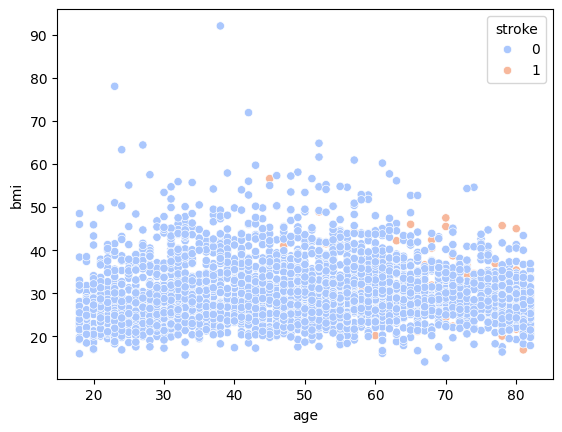
\includegraphics[scale=0.4]{Images/age_bmi_plot.png}
\caption{Age-BMI correlation plot}
\label{fig:age_bmi}
\end{subfigure}

\begin{subfigure}[b]{\linewidth}
\centering
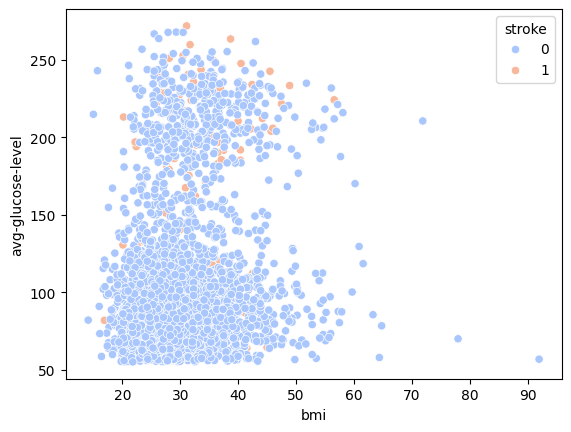
\includegraphics[scale=0.4]{Images/bmi-glucose_plot.png}
\caption{BMI-Glucose correlation plot}
\label{fig:bmi_glucose}
\end{subfigure}
\end{figure}

Following in the analysis, \ref{fig:age_glucose}. \ref{fig:bmi_glucose} and \ref{fig:age_bmi} plot the correlation between the numerical features inside the dataset. We can clearly see no linear dependencies in these plots, but it is evident a correlation between age and the incidence of higher values of blood sugar, that also seems to lead to a higher incidence of stroke. Interestingly, the 25-40 bmi values(overweight, obese I) seems to be the range in which the higher glucose levels are concentrated. However, this is also the range in which we have most of the samples.

\subsubsection{Balanced dataset}
After oversampling the dataset, we will show the plots of some of the features of the dataset, to understand better which one are more influential than others in predicting stroke.

\begin{figure}[h]
\centering
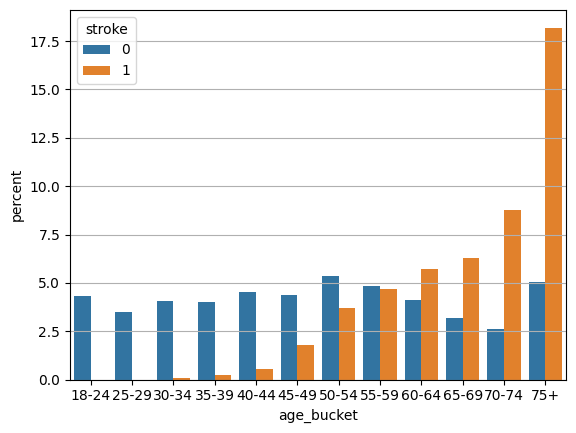
\includegraphics[scale=0.4]{Images/age_graph.png}
\caption{Age graph balanced dataset}
\label{fig:age_balanced}
\end{figure}

The age group graph (Figure \ref{fig:age_balanced}) shows the percentage of stroke occurrences across different age buckets. We observe that stroke incidence increases significantly with age, particularly in the 75+ age group, which has the highest stroke rate. This indicates that age is a critical factor in stroke risk.

\begin{figure}[h]
\centering
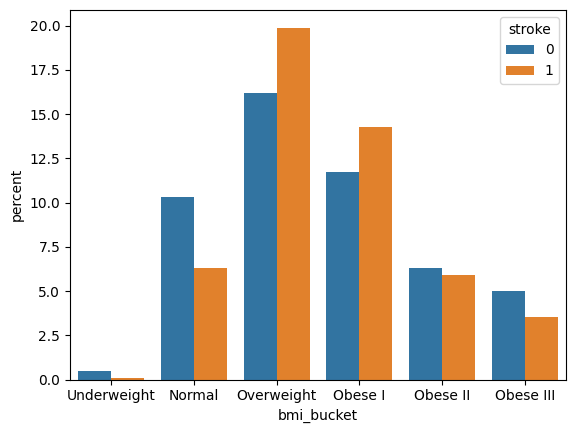
\includegraphics[scale=0.4]{Images/bmi_graph.png}
\caption{BMI graph balanced}
\label{fig:bmi_balanced}
\end{figure}

The BMI category graph (Figure \ref{fig:bmi_balanced}) illustrates the distribution of stroke occurrences across different BMI categories. Overweight and Obese I categories show a higher percentage of stroke patients compared to other BMI groups.

\begin{figure}[h]
\centering
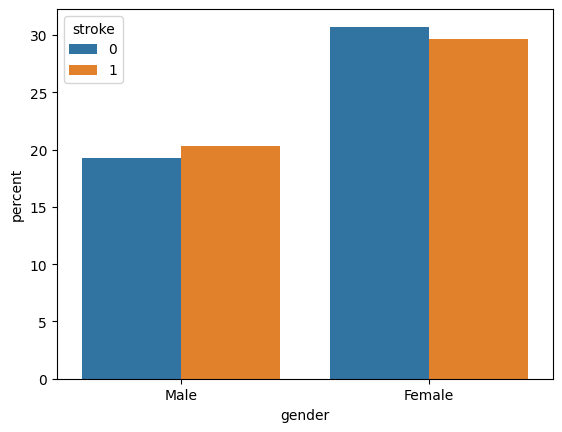
\includegraphics[scale=0.4]{Images/gender_graph.png}
\caption{Gender influence}
\label{fig:gender}
\end{figure}

The gender graph (Figure \ref{fig:gender}) presents the percentage of stroke occurrences among males and females. The data shows a slightly higher stroke rate in females compared to males, indicating potential gender-related risk factors for stroke.

\begin{figure}[h]
\centering
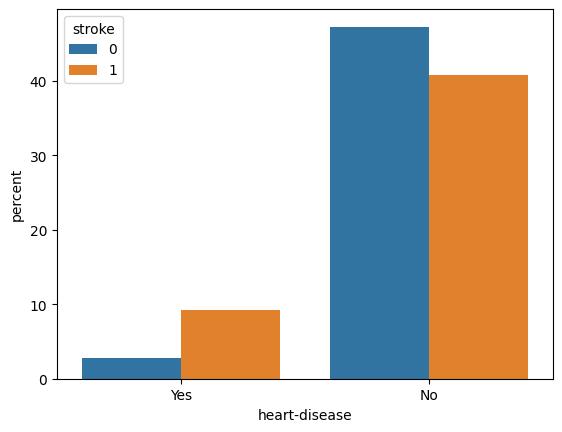
\includegraphics[scale=0.4]{Images/heart_disease_graph.png}
\caption{Heart disease incidence}
\label{fig:heart}
\end{figure}

The heart disease graph (Figure \ref{fig:heart}) shows the percentage of stroke occurrences among patients with and without heart disease. Patients with heart disease have a higher stroke rate, however it is also shown that most of the patients suffering from stroke, did not seem to suffer from heart disease. This highlights the importance of monitoring cardiovascular health to prevent strokes.

\begin{figure}[h]
\centering
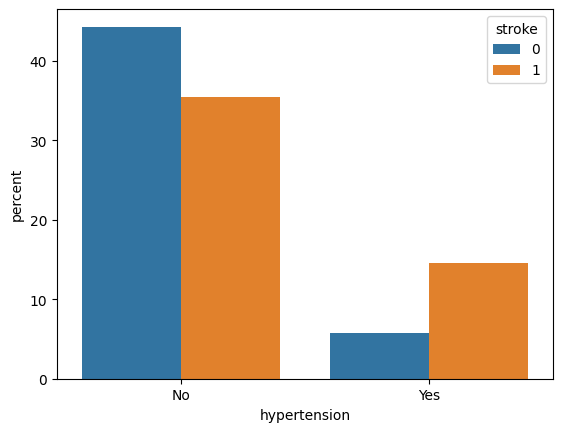
\includegraphics[scale=0.4]{Images/hypertension_graph.png}
\caption{Hypertension incidence}
\label{fig:hypertension}
\end{figure}

A similar argument can be drawn from \ref{fig:hypertension} that apparently does not contribute so much to the stroke class, but this can be explained as a lack of screening.

\begin{figure}[h]
\centering
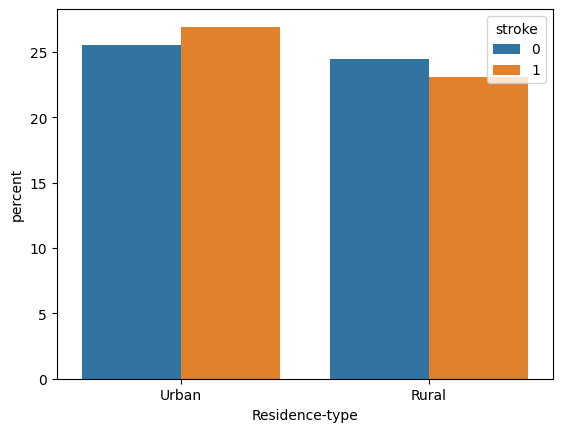
\includegraphics[scale=0.4]{Images/residence_type_graph.png}
\caption{Residence type incidence}
\label{fig:residence}
\end{figure}


The plot \ref{fig:residence} shows no significant stroke imbalance between living in a urban area or in the country side. So we are expecting this feature to have less importance in the model training.


\begin{figure}[h]
\centering
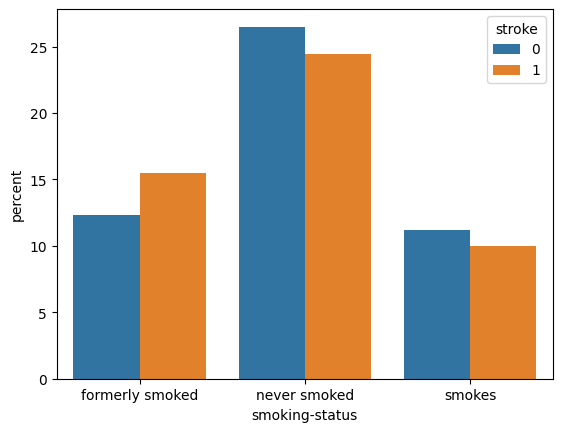
\includegraphics[scale=0.4]{Images/smoking_status_graph.png}
\caption{Smoking incidence}
\label{fig:smoking}
\end{figure}

The smoking status graph (Figure \ref{fig:smoking}) displays the stroke occurrences among patients with different smoking habits. Surprisingly, former smokers and never smokers show higher stroke rates compared to current smoker. Nonetheless, this trend may also be biased by the uneven distribution of the data.

\begin{figure}[h]
\centering
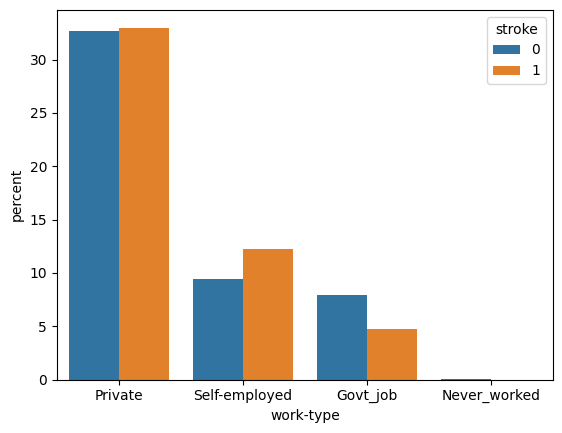
\includegraphics[scale=0.4]{Images/work_type_graph.png}
\caption{Work incidence}
\label{fig:work}
\end{figure}

The work type graph (Figure \ref{fig:work}) shows the distribution of stroke occurrences across different employment sectors. The private sector has the highest stroke rate, potentially due to higher representation in the dataset. Self-employed individuals also show a notable stroke rate.

\subsection{Feature Ranking}

In this section, we show the graphs of features obtained both for the paper replica and the best practice analysis. The results are very similar both for notebook A and B, so we will represent only the results for A. As also shown in the original paper, the Age feature is the most influential one, both for the information gain and Random Forest methods.

\begin{figure}[ht]
\centering
    \begin{subfigure}[b]{\linewidth}
    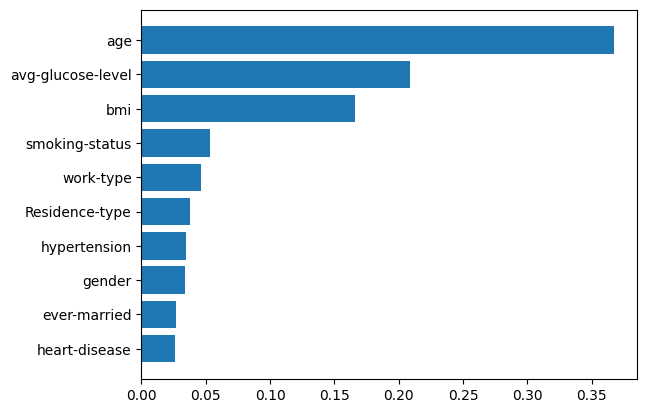
\includegraphics[scale=0.4]{Images/feature_ranking_random_forest.png}
    \caption{Random forest feature ranking}
    \label{fig:feature_ranking_forest}
    \end{subfigure}
    
    \begin{subfigure}[b]{\linewidth}
    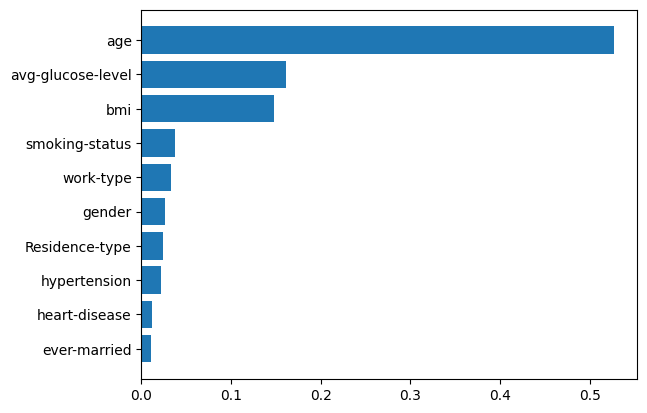
\includegraphics[scale=0.4]{Images/feature_ranking_info_gain.png}
    \caption{Information gain feature ranking}
    \label{fig:feature_ranking_information}
    \end{subfigure}
    
    \begin{subfigure}[b]{\linewidth}
    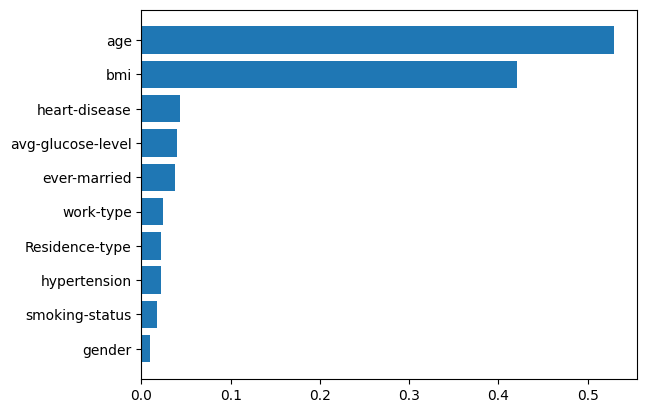
\includegraphics[scale=0.4]{Images/mutual_information_gain.png}
    \caption{Mutual information feature ranking}
    \label{fig:feature_ranking_mutual_info}
    \end{subfigure}
\end{figure}

\ref{fig:feature_ranking_forest} and \ref{fig:feature_ranking_information} depict the importance of each feature, computed using both a Random Forest Classifier and for the Information Gain method. Both methods indicate that age is the most relevant feature, other features such as bmi and average glucose level have an high rank in both methods. The information gain method was applied fitting a decistion tree, using 'entropy as criterion'. Out of curiosity also the mutual information score for the features were calculated. This technique computes the statistical correlation between the feature and the output labels. The result of the latter is shown in \ref{fig:feature_ranking_mutual_info} which also includes age and bmi among the most important features.


\section{Model Training and Evaluation}

In this section, we detail the models employed in our study, the methods used for hyperparameter tuning, and the evaluation metrics used to assess model performance.

\subsection{Model training}
We employed several machine learning models to predict stroke risk, following the methodology outlined in the original paper. The models used in our study include:

\begin{itemize}
    \item Logistic Regression
    \item Decision Tree Classifier
    \item Random Forest Classifier
    \item STochastic Gradient Descent (SDG) Classifier
    \item k-Nearest Neighbors (k-NN) Classifier
    \item Gaussian Naive Bayes
    \item Multi Layer Perceptron (MLP) Classifier 
    \item Stacking Classifier
    \item Majority Voting Classifier
\end{itemize}

Each model was trained on the preprocessed dataset using all the features. The stacking classifier, which combines a Gaussian Naive Bayes Classifier, a Random Forest Classifier and two decision trees imblementing both the Gini Criterion and Entropy criterion to split nodes in the classifier.

\subsection{Hyperparameter Tuning}
To optimize the performance of each model, we employed GridSearchCV for hyperparameter tuning. This method involves an exhaustive search over a specified parameter grid, evaluating each combination of parameters using cross-validation to identify the best-performing set.


We used GridSearchCV with 10-fold cross-validation to systematically explore the hyperparameter space for each model. This approach ensures that the selected hyperparameters provide the best generalization performance on unseen data.


The hyperparameter grids for each model were defined based on common practices and literature, ensuring a comprehensive exploration of the parameter space. The optimal hyperparameters identified through this process were then used to train the final models.

\subsection{Evaluation Metrics}
To evaluate the performance of the trained models, we used a variety of metrics, including:

\begin{itemize}
    \item \textbf{Accuracy}: The ratio of correctly predicted instances to the total instances.
    \item \textbf{Precision}: The ratio of true positive predictions to the sum of true positive and false positive predictions.
    \item \textbf{Recall}: The ratio of true positive predictions to the sum of true positive and false negative predictions.
    \item \textbf{F1-Score}: The harmonic mean of precision and recall, providing a single metric that balances both concerns.
    \item \textbf{Area Under the Curve (AUC)}: The area under the Receiver Operating Characteristic (ROC) curve, representing the model's ability to distinguish between classes.
\end{itemize}

These metrics provide a comprehensive evaluation of model performance, highlighting both the accuracy and the ability to correctly identify stroke occurrences.

\subsection{Results}

In this section we will present the results obtained from the model training. For simplicity, we will present only two matrices, each one refering to one notebook, that display the results obtained for each metric.

\subsubsection{Evalutation Methodology}

As already declared, we have developed two version of the notebook: version A tries to replicate the methodologies stated in the paper, while version B implements best practices. An important difference between version A and B is the dataset on which the models are tested on. In version A, since the whole dataset was augmented using the SMOTE technique, not only the train dataset but also the test one is balanced, this 'drugs' the metrics results, loosing the real world distribution of data. In version B we have decided to oversample only the train dataset, leaving the test dataset untouched, resulting in a more fair evalutaion of the model performance.

\begin{figure}[ht]
    \centering
    \begin{subfigure}[b]{\linewidth}
        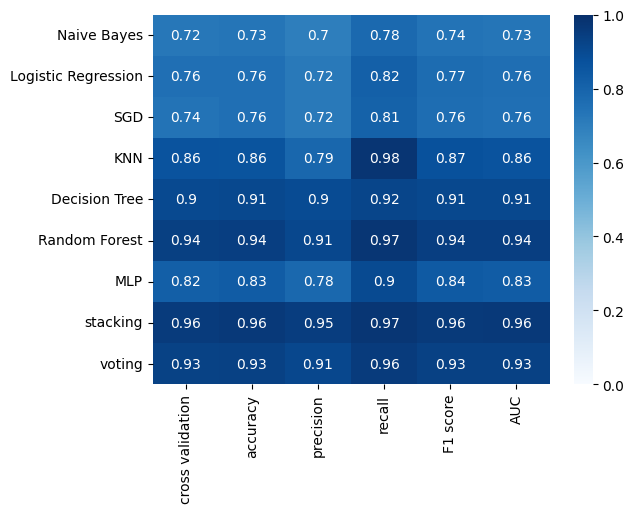
\includegraphics[scale=0.5]{Images/model_performance.png}
        \caption{Models performance A}
        \label{fig:eval_matrix_a}
    \end{subfigure}
    \begin{subfigure}[b]{\linewidth}
        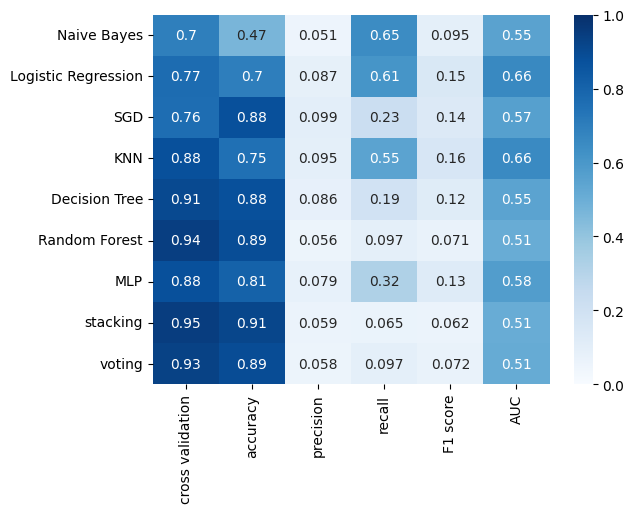
\includegraphics[scale=0.5]{Images/model_performance_b.png}
        \caption{Models performance B}
        \label{fig:eval_matrix_b}
    \end{subfigure}
\end{figure}

\subsubsection{Notebook A}

As we can clearly see from the matrix reported in \ref{fig:eval_matrix_a}, the results of each of the trained models seem to indicate a good model training. The models that performed overall best are the stacking, the random forest classifier and the majority voting ones with ROC AUC score of 96\%, 94\% and 93\%. For these models, also the recall metric seems to be pretty high. Having a high recall is foundamental when treating medical data, as it is better to have false positive than false negative in these cases and let other specialists double-check the data.

\subsubsection{Notebook B}

\ref{fig:eval_matrix_b} is showing another figure of the data instead. When testing the algorithms on data coming from real world, we can clearly see that the performance in precision and recall drop significantly, showing that other models such as K-Nearest Neighbours and Logistic regression, may achieve better results in unseen data.

% FOURTH CHAPTER
% --------------------------------------------------------------------------
\chapter{Conclusions}

\section{Paper Replication}
In the first part of our project, we meticulously followed the procedures and algorithms outlined in the referenced paper. This replication allowed us to validate the findings and understand the underlying assumptions and methodologies employed by the original authors. The trends in our findings differ only slightly from those showed in the paper, and are mainly imputable to some hyperparameters used in the SMOTE function that we were not able to replicate.

This part confirms the Stacking method as the most performing one, followed by Random Forest and Majority Voting.

\section{Best Practices Implementation}
The second part of the project revolved around the implementation of best practices to handle outliers and implement a fairer evaluation of our trained modes. In this section we have registered severe underperformance of the models on the real data distribution, rising awareness. In particular, it was concerning the low recall score of the models on the unseen data.

This part shows new emerging best predictions such as KNN, Logistic Regression and Naive Bayes Classifiers, that are chosen based on their high AUC and recall scores.

\bibliography{sample}

\end{document}
